%!TEX root = ../vkr.tex

\section {Техники восстановления знаков}
Уменьшение контроля над входами является существенной проблемой, которая затрудняет восстановление знаков в более глубоких слоях. Опишем эту проблему более подробно.

Пусть $\mathnormal{x} \in \mathbb{R}^{d_{0}}$ я вляется входом для DNN. $\mathnormal{F}_{\mathnormal{x}}^{\left(i-1\right)}$ и $\mathnormal{G}_{\mathnormal{x}}^{\left(i+1\right)}$ это свёрнутые матрицы для $\mathnormal{x}$, соответствующие уже восстановленной и ещё не известной части DNN, соответственно.
\Def{Пространство контроля для слоя $i$ вокруг входа $\mathnormal{x}$, обозначаемое $\mathnormal{V}_{\mathnormal{x}}^{\left(i-1\right)}$, это диапозон линейной трансформации  $\mathnormal{F}_{\mathnormal{x}}^{\left(i-1\right)}$. Размерностью этого пространства называется число степеней свободы для слоя $i$ со входом $\mathnormal{x}$ и обозначается  $\mathnormal{d}_{\mathnormal{x}}^{\left(i-1\right)}$.}

Пространство контроля это векторное пространство, содержащее все возможные малые измененния на входе в слой $i$, и, по определению, $\mathnormal{d}_{\mathnormal{x}}^{\left(i-1\right)} = \rank\left(\mathnormal{F}_{\mathnormal{x}}^{\left(i-1\right)}\right)$. Если в слоях с 1-ого по $i-1$ ReLU делает нейроны неактивными, то для фиксированного числа $\mathnormal{x}$ число степеней свободы останется равным или уменьшается с ростом $i$. Рассмотрим вход $\mathnormal{x}$, делающий половину от $d$ нейронов в 1-ом слое активными. Матрица $\mathnormal{F}_{\mathnormal{x}}^{\left(1\right)}$ тогда будет иметь ранг $d/2$, и, в частности, строки, соответствующие неактивным нейронам, являются нулевыми векторами. Если во втором слое $d' < d/2$ активных нейронов (для того же входа $\mathnormal{x}$), матрица $\mathnormal{F}_{\mathnormal{x}}^{\left(2\right)}$ имеет ранг $d'$, и, следовательно, число степеней свободы также равно $d'$. Теперь, если $d' \ge d/2$, то $\mathnormal{F}_{\mathnormal{x}}^{\left(2\right)}$ имеет ранг $d/2$ (поскольку ранг $\mathnormal{F}_{\mathnormal{x}}^{\left(1\right)}$ не может увеличиться при умножении на другую матрицу). Для последующих слоёв ситуация та же: ранг нельзя увеличить, если он уменьшился. По факту, число степеней свободы на слое $i$ обычно определяется минимальным числом активных нейронов на слой, среди всех слоёв от 1 до $i-1$, но в некоторых случаях, оно может быть строго меньше.

\begin{figure}[h]
	\centering{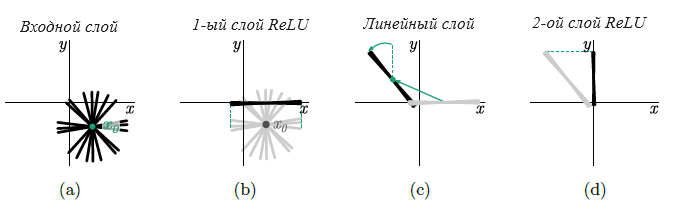
\includegraphics[width=1\linewidth]{control-s}}
	\caption{Интуиция для пространства контроля. Рассмотрим сеть с двумерным входом и двумя скрытыми слоями с двумя нейронами в каждом. (a) Для первого скрытого слоя пространство контроля $-$ это полное двумерное пространство. Мы можем перемещаться по входу $\mathnormal{x}_{0}$ в любом направлении. (b) После первого скрытого слоя, если один ReLU положительный, а другой отрицательный, мы теряем одно измерение контроля. (c) Линейное преобразование во втором слое будет вращать, перемещать и масштабировать пространство контроля. (d) Таким образом, после ReLU во стором слое(если опять же один положительный, а другой отрицательный) у нас остаётся одномерное пространство контроля. При отсутствии вращения пространство контроля сворачивается в точку после этих двух скрытых слоёв.}
	\label{ris:control-s}
\end{figure}

Расмотрим DNN с входной размерностью $d$ и одинаковой шириной $d$ во всех скрытых слоях. Предположим далее, что каждый нейрон имеет вероятность $1/2$ быть активным. Изначально число степеней свободы равно размерности $d$ входа DNN. Затем в первом скрытом слое будет активна в среднем половина нейронов, что уменьшит число степеней свободы на входе слоя 2 до $d/2$. Можно считать, что ReLU проецирует пространство контроля на пространство, определяемое активными нейронами. Можно подумать, что половина из этих $d/2$ степеней свободы снова будет потеряна во втором слое из-за того, чо половина его ReLU будет неактивна, и в итоге получится $d/4$ степеней свободы. Однако, прежде чем перейти к ReLU на этом слое, пространство контроля для слоя 2 обычно поворачивается за счёт $A^{\left(2\right)}$. благодаря этому повороту многие координаты могут пережить проекцию ReLU на второй слой. Мы всё ещё можем потерять несколько степеней свободы, но не более половины из них на каждом последующем слое. Благодаря этому эффекту линейного преобразования число степеней свободы обычно стабилизируется после нескольких первых слоёв. На рисунке $\ref{ris:control-s}$ это явление изображено в двумерном случае.

В контексте атаки при восстановлении знаков слоя $i$ мы полностью знаем $\mathnormal{F}_{i-1}$, знаем $\mathnormal{f}_{i}$ с точностью до знака на нейрон, и $\mathnormal{G}_{i+1}$ полностью неизвестно. Для простоты записи опустим подстрочный индекс $\mathnormal{x}$

\subsection{Восстановление знаков SOE}
Рассмотрим случай, когда число степеней свободы достаточно велико. Название метод SOE получил, так как он основан на решении системы уравнений (\textbf{S}ystem \textbf{O}f \textbf{E}quations). Этот метод внешне похож на метод "Замораживания", но использует другие уравнения и другой набор переменных (в случае "Замораживания" переменные обозначали направление, по которому мы должны двигаться во входжном пространстве, чтобы "заморозить" все нейроны кроме целевого, в то время как в SOE переменные обозначают коэффициенты выходной функции $\mathnormal{G}_{i+1}$ в некоторой случайно выбранной точке $\mathnormal{x}$). 

Как и прежде, пусть $I_{\mathnormal{x}}^{\left(i\right)} ~-$  матрица, представляющая ReLU на лое $i$ для входа $\mathnormal{x}$. Уравнение для изменения выхода при произвольной последовательности изменений входа $\mathit{\Delta}_{k}$, может быть записано как
$$\mathnormal{f}\left(\mathnormal{x} + \mathit{\Delta}_{k}\right) - \mathnormal{f}\left(\mathnormal{x}\right) = \mathnormal{G}_{\mathnormal{x}}^{\left(i+1\right)} {I}_{\mathnormal{x}}^{\left(i\right)} A^{\left(i\right)} \mathnormal{F}_{\mathnormal{x}}^{\left(i-1\right)} \mathit{\Delta}_{k}.$$

Пусть, $y_{k} = A^{\left(i\right)} \mathnormal{F}_{\mathnormal{x}}^{\left(i-1\right)} \mathit{\Delta}_{k}$ и $c =  \mathnormal{G}_{\mathnormal{x}}^{\left(i+1\right)} {I}_{\mathnormal{x}}^{\left(i\right)}$. Если соблюдается левосторонность наблюдается в полученни значений $z_{k}$ через прямые запросы, уравнение может быть переписано в виде
$$c \cdot y_{k} = z_{k},$$
которое можно рассматривать как систему уравнений, где $c ~-$ вектор переменных. В силу ReLU, если нейрон $j$ неактивен на входе $\mathnormal{x}$, то $c_{j}=0$, поэтому получив $d_{i}$ уравнений, мы можем решить систему и определить, какие нейроны неактивны в окрестности $\mathnormal{x}$, и, следовательно, выбрать подходящие знаки для текущего слоя.
\begin{remark}
В контексте атаки мы можем восстановить $y_{k}$ только до глобального масштабирования каждого входа (включая, возможно, перестановку знаков), но это приводит к системе уравнений, в которой решение имеет тот же набор исчезающих переменных.
\end{remark}
\textbf{Вызовы Оракула/Время.} Данный метод оптимален с точки зрения количества запросов, так как для решения слоя размера $d_{i}$ требуется только $d_{i}+1$ запрос (а именно, нужно запросить $\mathnormal{f}\left(\mathnormal{x}\right)$ и $\mathnormal{f}\left(\mathnormal{x} + \mathit{\Delta}_{k}\right)$ для $d_{i}$ значений $k$). После выполнения запросов временная сложность атаки заключается в решении системы уравнений, что можно сделать за $\mathcal{O}\left(d_{i}^{3}\right)$ с помощью стандартных методов.

\textbf{Ограничения.} Каждый выбор $\mathit{\Delta}_{k}$ приводит к новому уравнени, поэтому мы пытаемся собрать больше уравнений, пока система не станет однозначно разрешимой. Однако не все полученные уавнения могут быть линейно независимыми. На самом деле, поскольку все $\mathnormal{y}_{k}$ лежат в $A^{\left(i\right)}\left(V_{\mathnormal{x}}^{\left(i-1\right)}\right)$, мы получим достаточно линейно независимых уравнений, только если $d_{\mathnormal{x}}^{\left(i-1\right)} \ge d_{i}$. Вероятно, так и будет, если размер слоя будет постоянно уменьшаться в 2 раза, но есть важное исключение для первых двух скрытых слоёв. Действительно, пока сеть не расширяется, линейная карта, соответствующая первому скрытому слою может быть инвертирована. Это позволяет легко найти $\mathnormal{x}$,  при котором все нейроны первого слоя активны, и следовательно, $d_{\mathnormal{x}}^{\left(1\right)}  = d_{1} \ge d_{2}$. Таким образом, метод легко применим для первых двух скрытых слоёв при единственном условии $-$ отсутствии расширеи, а в последующих слоях он может быть успешен только в том случае, если каждый из них уменьшится на коэффициент, близкий к 2.

\subsection{Восстановление знака колебанием нейронов}
Данный метод не имеет таких жестких ограничений на архитектуру сети, как описанный выше, поскольку его производительность постепенно снижается по мере уменьшения числа степеней свободы, в то время как в SOE система уравнений резко переходит от разрешимой к неразрешимой.
\Def{Колебание на $i$-ом слое это вектор $\delta \in \mathbb{R}^{d_{i-1}}$ разностей значений нейронов в этом слое.}
Вспомним, что восстановленная матрица весов для слоя $i$ это $\hat{A}^{\left(i\right)} \in \mathbb{R}^{d_{i} \times d_{i-1}}$ и пусть её $k$-ая строка это $\hat{A}_{k}^{\left(i\right)}$. Для колебания $\delta$ в слое $i$, нейрон $k \in \{1, \dots, d_{i}\}$ в этом слое изменяет своё значение на $e_{k} = \left \langle \hat{A}_{k}^{\left(i\right)}, \delta \right \rangle$. Рассмотрим один выход DNN, и пусть $\left(c_{1}, \dots, c_{d_{i}}\right) ~-$ это соответствующий ему вектор выходных коэффициентов (т.е. соответствующий вектор-строка в $\mathnormal{G}^{\left(i+1\right)}$). Если мы "протолкнём"\ разность $e_{k}$ через оставшиеся слои, то разность на выходе будет 
\begin{equation}
  \label{eq2} \sum_{k \in I} {c_{k} e_{k}},
\end{equation}
где $I$ содержит индексы всех активных нейронов слоя $i$. Мы хотим восстановить знак нейрона $j$. Если этот нейрон активен, выходная разность содержит вклад $e_{j}$. Если нейрон неактивен, ReLU "блокирует"\ $e_{j}$, и он не вносит свой вклад. Когда $c_{j} e_{j}$ достаточно велико, мы можем определить, присутствует ли он в $\ref{eq2}$, и использовать эту информацию для фосстановления знака нейрона. Лучше всего это получается, когда $\delta ~-$ это колебание, которе максимизирует изменение значения для данного нейрона, т.е. $\left \| \hat{A}^{\left(i\right)} \delta \right \|_{\infty} = \left | e_{j} \right |$. Важнейшее свойство, которое мы здесь получаем, состоит в том, что максимизация размера колебания, производимого линейным выражением, не требует знания его знака $-$ если мы отрицаем выражение, то получаем колебание того же размера, но в противоположном направлении. Теперь покажем, как вычислить такое максимальное колебание и как восстановить знак целевого нейрона.

\textbf{Вычисление колебания целевого нейрона.} Пусть $\delta \in \mathbb{R}^{d_{i-1}}$ параллельно $\hat{A}_{j}^{\left(i\right)}$ (т.е. все координаты $\delta$ имеют тот же, либо противоположный знак к соответствующей координате  $\hat{A}_{j}^{\left(i\right)}$). Тогда все слагаемые в скалярном произведении $\left \langle \hat{A}_{j}^{\left(i\right)}, \delta \right \rangle$ имеют одинаковый знак. Если ни одна строка в  $\hat{A}^{\left(i\right)}$ не кратна  $\hat{A}_{j}^{\left(i\right)}$, тогда с высокой вероятностью $\left | \left \langle \hat{A}_{j}^{\left(i\right)}, \delta \right \rangle \right | > \left | \left \langle \hat{A}_{k}^{\left(i\right)}, \delta \right \rangle \right |$, для всех $k \not = j.$ Это значит, что $\left \| \hat{A}^{\left(i\right)} \delta \right \|_{\infty} = \left | \left \langle \hat{A}_{j}^{\left(i\right)}, \delta \right \rangle \right |$. Следовательно, изменение значения для нейрона $j$ может быть максимальным, если колебание параллельно $ \hat{A}_{j}^{\left(i\right)}$.

$V^{\left(i-1\right)} ~-$ это пространство контроля для слоя $i$ при входном сигнале $\mathnormal{x}$. Мы проецируем $ \hat{A}_{j}^{\left(i\right)}$ на $V^{\left(i-1\right)}$ и получаем $\delta$, масштабируя эту проекцию так, чтобы она имела достаточно малую норму $\epsilon^{\left(i-1\right)}$. Наконец, мы получаем входную разность $\mathit{\Delta} \in \mathbb{R}^{d_{0}}$, которая порождает $\delta$, найдя прообраз $\delta$ под $\mathnormal{F}^{\left(i-1\right)}$.

\textbf{Восстановление знака целевого нейрона.} Вы хотим восстановить знак для $\eta_{j} ~-~j$-ого нейрона в слое $i$. Пусть $\mathnormal{x}^{*} ~-$ критическая точка для $\eta_{j}$ и пусть $\mathit{\Delta} \in \mathbb{R}^{d_{0}}$ генерирует колубание $\delta$ (на слое $i$), которое максимизирует изменение значеня для этого нейрона. Предположим, что знак $\eta_{j}$ положительный. Тогда знаки восстановленных весов $\hat{A}_{j}^{\left(i\right)}$ такие же  как и у настоящих весов  ${A}_{j}^{\left(i\right)}$. Отсюда следует, что и координаты $\delta$ имеют тот же знак, что и координаты  ${A}_{j}^{\left(i\right)}$ и $e_{k} = \left \langle {A}_{k}^{\left(i\right)}, \delta \right \rangle$ имеет положительное значение. Поскольку $\mathnormal{x}^{*}$ является критической точкой для $\eta_{j}$, вычисление DNN в точке $\mathnormal{x}^{*} + \mathit{\Delta}$ делает нейрон $\eta_{j}$ активным, таким образом
$$\mathnormal{f}\left(\mathnormal{x}^{*} + \mathit{\Delta}\right) - \mathnormal{f}\left(\mathnormal{x}^{*}\right) = c_{j} e_{j} + \sum_{k \in I \setminus \{j\}} {c_{k} e_{k}},$$
где $I ~-$ индексы всех активных нейронов слоя $i$. Необходимо, чтобы $\mathit{\Delta}$ изменял состояние только нейрона $\eta_{j}$. При вычислении в точке $\mathnormal{x}^{*} - \mathit{\Delta}$ колебание $\delta$ имеет противоположные знаки, чем ${A}_{j}^{\left(i\right)}$. Тогда, все разности $e_{k}$ также имеют противоположные знаки(в сравнении со значениями в $\mathnormal{x}^{*} + \mathit{\Delta}$). В данном случае, $\eta_{j}$ становится неактивным и мы имеем что
$$\mathnormal{f}\left(\mathnormal{x}^{*} - \mathit{\Delta}\right) - \mathnormal{f}\left(\mathnormal{x}^{*}\right) = - \sum_{k \in I \setminus \{j\}} {c_{k} e_{k}}.$$
Теперь предположим, что $\eta_{j}$ имеет отрицательный знак. Тогда колебания $\delta$ будут иметь противоположные знаки, чем  ${A}_{j}^{\left(i\right)}$, и, следуя аналогичному анализу, мы получим, что 
$$\mathnormal{f}\left(\mathnormal{x}^{*} + \mathit{\Delta}\right) - \mathnormal{f}\left(\mathnormal{x}^{*}\right) = - \sum_{k \in I \setminus \{j\}} {c_{k} e_{k}}$$
и
$$\mathnormal{f}\left(\mathnormal{x}^{*} - \mathit{\Delta}\right) - \mathnormal{f}\left(\mathnormal{x}^{*}\right) = c_{j} e_{j} + \sum_{k \in I \setminus \{j\}} {c_{k} e_{k}}.$$
Таким образом, чтобы определить знак, нам нужно определить, вносит ли $c_{j} e_{j}$ вклад в выходную разность с $\mathnormal{x}^{*} - \mathit{\Delta}$ или $\mathnormal{x}^{*} + \mathit{\Delta}$.

Пусть $L = \mathnormal{f}\left(\mathnormal{x}^{*} - \mathit{\Delta}\right) - \mathnormal{f}\left(\mathnormal{x}^{*}\right)$ и $R = \mathnormal{f}\left(\mathnormal{x}^{*} + \mathit{\Delta}\right) - \mathnormal{f}\left(\mathnormal{x}^{*}\right)$ обозначают, соответственно, выходную разность слева и справа для $\mathnormal{x}^{*}$. Мы решаем, что $c_{j} e_{j}$ появляется слева, т.е. знак нейрона равен $-1$, если $|L|>|R|$. Иначе, мы решаем, что знак равен $+1$.  Так как $c_{j} e_{j} \not = 0$, то невозможно, что $|L|=|R|$.

Если $c_{j} e_{j}$ и $\sum \nolimits_{k}{c_{k} e_{k}}$ имеют одинаковый знак, тогда $\left |c_{j} e_{j} + \sum \nolimits_{k}{c_{k} e_{k}} \right| > \left|-\sum \nolimits_{k}{c_{k} e_{k}}\right|$ всегда выполняется, и решение о знаке всегда верно. Если $c_{j} e_{j}$ и $\sum \nolimits_{k}{c_{k} e_{k}}$ имеют противоположные знаки, это может привести к неправельному решению. Это неправильное решение случается, когда  $\left|-\sum \nolimits_{k}{c_{k} e_{k}}\right| > \left |c_{j} e_{j} + \sum \nolimits_{k}{c_{k} e_{k}} \right|$. Тогда для правильного решения необходимо, чтобы  $\left |c_{j} e_{j}\right| > 2 \left|\sum \nolimits_{k}{c_{k} e_{k}}\right|$.

Вспомним, что заданный вход DNN определяет частичную матрицу $\mathnormal{G}^{\left(i+1\right)}$. То есть, разные входы определяют разные коэффициенты на выходе DNN. Этот факт называется \textit{рандомизацией выхода} и используется он для преодоления проблемы принятия неверного решения о знаке. Мы находим $s$ различных критических точек для нейрона $\eta_{j}$; каждая точка определяет различные выходные коэффициенты. Мы ожидаем, что большинство этих точек определяют такие коэффициенты, что $c_{j} e_{j}$ и $\sum \nolimits_{k}{c_{k} e_{k}}$ выполняют условия для принятия правильного решения. Для каждой критической точки, мы вычисляем колебание $\delta$, соответствующее входной разности $\mathit{\Delta}$, и делаем выбор знака. Пусть $s_{-}$ и $s_{+}$ обозначают, соответственно, число критических точек, для которых знак был выбран $-1$ и $+1$. Также, пусть \textit{уровень доверия} $\alpha$ для $-1$ равен ${s_{-} / s}$ и $s_{+} / s$ для $+1$. Затем принимаем решение о знаке $-1$, если $s_{-} > s_{+}$, и уровень доверия больше, чем порог $\alpha_{0}$. Если $s_{+}>s_{-}$ и уровень доверия больше, чем $\alpha_{0}$, то принимаем решение о $+1$. Иначе, решение о знаке не делается. В последнем случае, мы можем попробовать воостановить знак при помощи дополнительных критических точек.

С увеличением числа нейронов техника станет ещё лучше, поскольку в более высоких измерениях векторы, как правило, более ортогональны друг другу, и, следовательно, соотношение между размерами колебанй в целевом нейроне и в других нейронах должно увеличиться.

До сих пор мы предполагали, что у DNN один выход. Когда у неё несколько выходов, мы можем использовать евклидову норму над вектором выходов для сравнения $L$ и $R$, что выгодно для данного метода. Это связано с тем, что каждая критическая точка рандомизирует коэффициенты нескольких выходов, и вероятность того, что несколько выходов будут иметь одновременно "плохие" коэффициенты, ниже.

\textbf{Вызов оракула/Время.} Чтобы восстановить знак одного нейрона для $s$ критических точек, мы вычисляем $\mathit{\Delta}$ и сравниваем $L$ с $R$. Вычислене $\mathit{\Delta}$ не требует запросов к оракулу: для этого достаточно выполнить операции линейной алгебры, чтобы найти критическую точку $\mathnormal{x}^{*}$, спроецировать  ${A}_{j}^{\left(i\right)}$ на $V^{\left(i\right)}$ и найти $\mathit{\Delta}$. В частности, умножения и инверсии матриц. Размер задействованных матриц определяется количеством входов $d_{0}$ и числом нейронов $d_{i}$. Таким образом, временная сложность составляет $\mathcal{O}\left(d^{3}\right)$, где $d = \max(d_{0}, d_{i})$. Сравнение $L$ с $R$ требует запросов к оракулу на $\mathcal{x}^{*}$,  $\mathcal{x}^{*} - \mathit{\Delta}$ и $\mathcal{x}^{*} + \mathit{\Delta}$. Вычисление  $L =\left \| \mathnormal{f}\left(\mathnormal{x}^{*} - \mathit{\Delta}\right) - \mathnormal{f}\left(\mathnormal{x}^{*}\right) \right \|$ и $R = \left \| \mathnormal{f}\left(\mathnormal{x}^{*} + \mathit{\Delta}\right) - \mathnormal{f}\left(\mathnormal{x}^{*}\right) \right \|$ требует $\mathcal{O}(d_{r+1})$ операций, где $d_{r+1}$ это число выходов DNN. Таким образом, для одного нейрона требуется $3s$ запросов и $\left(s d^{3}\right)$ операций. В общей сложности нам потребуется $3sd_{i}$ запросов и $\mathcal{O}\left(sd_{i}d^{3}\right)$ операций для восстановления знака всех нейронов в слое $i$.

\textbf{Ограничения.} Мы можем рассматривать $c_{j} e_{j}$ как сигнал, а $\sum \nolimits_{k}{c_{k} e_{k}}$ как шум. Мы видели, что когда знаки сигнала и шума различаются, мы можем ошибочно определить знак нейрона. Это происходит, когда сигнал недостаточно велик по сравнению с шумом. В частности, если количество нейронов в слое $i$ слишком велико по сравнению со степенями свободы (для конкретного входа $\mathnormal{x}$), сигнал может быть очень слабым по отношению к шум. Это означает, что данная техника может не работать с DNN с большим расширением по сравнению с наименьшим скрытым слоем или количеством входов.

Кроме того, этот метод может не подойти для DNN с небольшим количеством нейронов в целевом слое. Вероятность того, что два случайных вектора будут перпендикулярны, уменьшается в низкоразмерных пространствах. Поэтому колебание для целевого нейрона может привести к ощутимо большим изменениям и для других нейронов (с весовыми векторами, несколько параллельными весовым векторам целевого нейрона). В этой ситуации вклад других нейронов может противодействовать вкладу целевого нейрона.

Наконец, этот метод использует рандомизацию вывода. При восстановлении последнего скрытого слоя рандомизация выходов отсутствует. Если в этом слое есть нейроны с плохими (постоянными коэффициентами, то соответсвтующий им знак будет восстановлен неверно.

\subsection{Восстановление знака последнего скрытого слоя}
Данный метод сосредоточен на восстановлении знака нейронов в последнем скрытом слое. Выход DNN представляется как аффинное преобразование $\mathnormal{f}_{r+1}$ без последующих вызовов ReLU. Поэтому, в слое $r$ (последний скрытый слой), матрица $G^{\left(r+1\right)}$ одинакова для всех входов $\mathnormal{x}$. Это означает, что все входы определяют одинаковые выходные коэффициенты; эквивалентно, для этого слоя не существует рандомизации выхода. Мы используем этот факт, чтобы восстановить знаки нейронов. Выходные коэффициенты восстанавливаются через вторые производные, таким образом, этот метод напоминает дифференциальный криптоанализ второго порядка.

Пусть $c_{1}, \dots, c_{r} ~-$ выходные коэффициенты. Также, пусть $\mathnormal{x} ~-$ входной сигнал DNN и $\mathnormal{y}^{(i)}$ есть выход $i$-ого слоя после ReLU, т.е., $\mathnormal{y}^{(i)} = \mathnormal{F}_{i}(\mathnormal{x})$. Выходной сигнал DNN определяется как
\begin{equation}
	\label{eq3} \mathnormal{f(x)} = c_{1} y_{1}^{(r)} + \cdots + c_{d_{r}} y_{d_{r}}^{(r)} + b^{(r+1)},
\end{equation}
где $y_{k}^{(r)} ~-~k$-ая координата $y^{(r)}$ и $b^{(r+1)}~-$ смещение выходного слоя.

С помощью восстановленной матрицы $\hat{A}^{(r)}$, мы можем вычислять значение, которое примет $k$-ый нейрон в слое $r$ перед ReLU, то есть $e_{k} = \left \langle \hat{A}^{(r)}, y^{(r-1)} \right \rangle$, но мы не знаем его знак $s_{k}$. Рассмотрим оба варианта. Только один $e_k$ или $-e_{k}$ положительный, а другой $-$ отрицательный; последний будет заблокирован ReLU. Таким образом, $\sigma(e_{k}, -e_{k})$ это либо $(e_{k}, 0)$, либо $(0, e_{k})$, в зависимости от того $e_{k} > 0$ или $e_{k}<0$, соответственно. Мы знаем значение $e_{k}$, поэтому мы можем вычислить  $\sigma(e_{k}, -e_{k})$. Запишем $\left(\hat{y}_{k+}^{(r)},\hat{y}_{k-}^{(r)}\right) = \sigma(e_{k}, -e_{k})$ . Теперь, нахождение $s_{k}$ эквивалентно решению вещественное значение ${y}_{k}^{(r)}$ нейрона после ReLU равно $\hat{y}_{k+}^{(r)} $ или $\hat{y}_{k-}^{(r)}$. Вклад $\mathnormal{f(x)}$ в уравнении $\ref{eq3}$ это $c_{k} \hat{y}_{k+}^{(r)}$ когда $s_{k} = +1$, иначе это $c_{k} \hat{y}_{k-}^{(r)}$. Тогда это уравнение может быть переписано как
$$\mathnormal{f(x)}=\sum_{k=1}^{d_{r}}{c_{k} \left(s_{k} \hat{y}_{k+}^{(r)}+\left(1-s_{1}\right) \hat{y}_{k-}^{(r)}\right)}+b^{(r+1)}.$$
Итак, мы берём случайные входы $\mathnormal{x}$, строит систему линейных уравнений и решаем для неизвестных $s_{k}$ и $b^{(r+1)}$. Нам нужно выбрать не менее $d_{r}+1$ случайных входов, чтобы система имела единственное решение.

Выходные коэффициенты $c_{k}$ могут быть получены через вторую производную, которая представляет собой изменение наклона функции. Вторая производная для функции ReLU:
$$c = \frac{\sigma(y+\epsilon)-2\sigma(y)+\sigma(y-\epsilon)}{\epsilon^{2}}$$
Пусть $\mathnormal{x}^{*} ~-$ критическая точка $k$-го нейрона слоя $i$ и $\mathit{\Delta} ~-$ вектор малой норм в линейной окрестности  $\mathnormal{x}^{*}$. Тогда,
$$\mathnormal{f}\left(\mathnormal{x}^{*}+\mathit{\Delta}\right)-2\mathnormal{f(x^{*})}+\mathnormal{f}\left(\mathnormal{x}^{*}-\mathit{\Delta}\right)=\pm\left\langle\mathnormal{F}_{k}^{\left(i\right)},\mathit{\Delta}\right\rangle c_{k},$$
где $\mathnormal{F}_{k}^{\left(i\right)} ~-$ это $k$-ая строка матрицы $\mathnormal{F}^{\left(i\right)}$ определяемая $\mathnormal{x}^{*}$ при коллапсе слоёв с $1$-ого по $i$-ый. Знак выше "$+$"\ когда $\mathnormal{x}+\mathit{\Delta}$ активирует нейрон и "$-$"\ иначе. Если $\mathit{\Delta}$ параллелен $\mathnormal{F}_{k}^{\left(i\right)}$, $\left\langle\mathnormal{F}_{k}^{\left(i\right)},\mathit{\Delta}\right\rangle > 0$ и нейрон активирован с $\mathnormal{x}+\mathit{\Delta}$. Тогда, разделив полученное выше выражение на $\left\langle\mathnormal{F}_{k}^{\left(i\right)},\mathit{\Delta}\right\rangle$ получим коэффициент. При восстановлении знака мы не имеем доступ к настоящей  $\mathnormal{F}^{\left(i\right)}$, но мы знаем $\hat{\mathnormal{F}}^{\left(i\right)}=\hat{A}^{(i)}\mathnormal{F}^{(i-1)}$ Чтобы получить коэффициент $k$-ого нейрона мы выбираем $\mathit{\Delta}$ как $\hat{\mathnormal{F}}_{k}^{\left(i\right)}$ масштабированную так, чтобы норма была достаточно малой. Получение выходного коэффициента нейрона $k$  может быть выполненно для любого скрытого слоя. ТОлько в последнем из них коэффициенты остоются постоянными для разных точек $\mathnormal{x}^{*}$.

\textbf{Вызовы Оракула/Время.} Сначала для каждого нейрона мы находим критическую точку и вычисляем выходной коэффициент. Это требует $3$-ёх запросов к оракулу и операций линейной алгебры со сложностью по времени $\mathcal{O}\left(d^{3}\right)$, где $d=max\left(d_{0}, d_{r}\right)$. То есть для всех $d_{r}$ нейронов требуется $3d_{r}$ запросов и временная сложность $\mathcal{O}\left(d_{r} d^{3}\right)$. Тогда, построение системы уравнений также требует $\mathcal{O}\left(d^{3}\right)$ операций (чтобы вычислить значения $\hat{y}_{k-}^{(r)}$ и $\hat{y}_{k+}^{(r)}$ для $d_{r}+1$ точки) и $d_{r}+1$ запросов. Наконец, решение системы уравнений требует $\mathcal{O}_{r}\left(d^{3}\right)$ операций и не требует запросов.Всего нам требуется $4d_{r}+1$ запросов, а временная сложность составляет $\mathcal{O}\left(d_{r}d^{3}\right)$ операций.

\textbf{Ограничения.} Эта техника требует, чтобы выходные коэффициенты были постоянными. Это происходит только в последнем скрытом слое. Поэтому данный метод применим только к этому слою.